\chapter{Метод реинжиниринга информационных систем, использующих дмнамически формируемые выражения}

В данной главе изложен метод проведения реинжинирига информационных систем, использующих строковые встроенные языки (string-embedded languages~\cite{Alvor1}). Рассмотрены основные типы задач, решаемых при реинжиниринге, указаны особенности обработки встроенных языков при их решении. Основной акцент сделан на обработку динамически формируемого SQL-кода, однако изложенный метод может быть адаптирован к обработке систем, использующих другие встроенные языки.

\section{Особенности}

Реинжиниринг информационных систем как правило является комплексным мероприятием, которое может в ключать в себя различные шаги, такие как анализ кода и его изучение, его рефактоинг, трансформацию, перенос на другие программно-аппаратные платформы~\cite{reengANT}. При этом часто проводится комплексный анализ многокомпонентной системы целиком, что приводит к необходимости уитывать различные особенности системы и работать с разнородными артефактами: документацией, исходным кодом, конфигурационными скриптами, скриптами баз данных и т.д. Всвязи с высокой сложностью такого анализа, ренжиниринг, как правило, является автоматизированным, а не полностью автоматическим процесс, что означает возможность (и необходимость) активного участия человека. Это позволяет использовать инструменты, которые не приводят сразу к получению конечнго результата, однако минимизируют ресурсы, необходимые для решения задачи. Например, может оказаться, что в системе присутствуют файлы особого формата и для их автоматической обработки потребуется создание уникального инструмента, что потребует значительных ресурсов. Однако объём этих файлов мал и их ручной анализ прост. В ситуации, когда затраты на создание инструмента значительно выше затрат на ручной анализ с тем же качеством результата, часто оказывается выгоднее отказаться от создания инструмента.

С одной стороны, динамически формируемый код может содержать важную информацию о системе. Например, в динамически формируемых SQL-запросах могут содержаться сведения о схеме данных и особенностями работы с базой данных, не извлекаемые из внешнего кода. С другой стороны, при активном использовании динамически формируемый код является сущьностью, требующей отдельного внимания при обработке системы и, следовательно, должен быть учтён, например, при оценки сложности системы, часто проводимой на начальных этапах при определении сроков и стоимости работ.

Системы используют строковые встроенные языки с разной интенсивностью и разными способами. В зависимости от характера использования встроенных языков меняются требования к автоматизации их обработки: необходима ли инструментальная поддержка или ручная обработка потребует меньше ресурсов, чем создание или освоение инструмента, какими именно инструментами пользоваться в тех или иных случаях.

Метода не обнаружено. Надо предложить свой.


\section{Метод}

Как было сказано ранее, встроенным языком может оказаться любой язык, однако на практике достаточно широко распространено использование днамически формируемого SQL-кода и генерация HTML-страниц. Использование динамически формируемого кода на других языках встречается реже. По этим причинам далее описан метод реинжиниринга систем, использующих встроенный SQL, однако он может быть адаптирован и к обработке систем, использующих другие встроенные языки. Общая последовательность шагов метода представлена на рисунке~\ref{fig:method}, а детальное описание шагов приведено далее.

\begin{figure}[h!]
\begin{center}
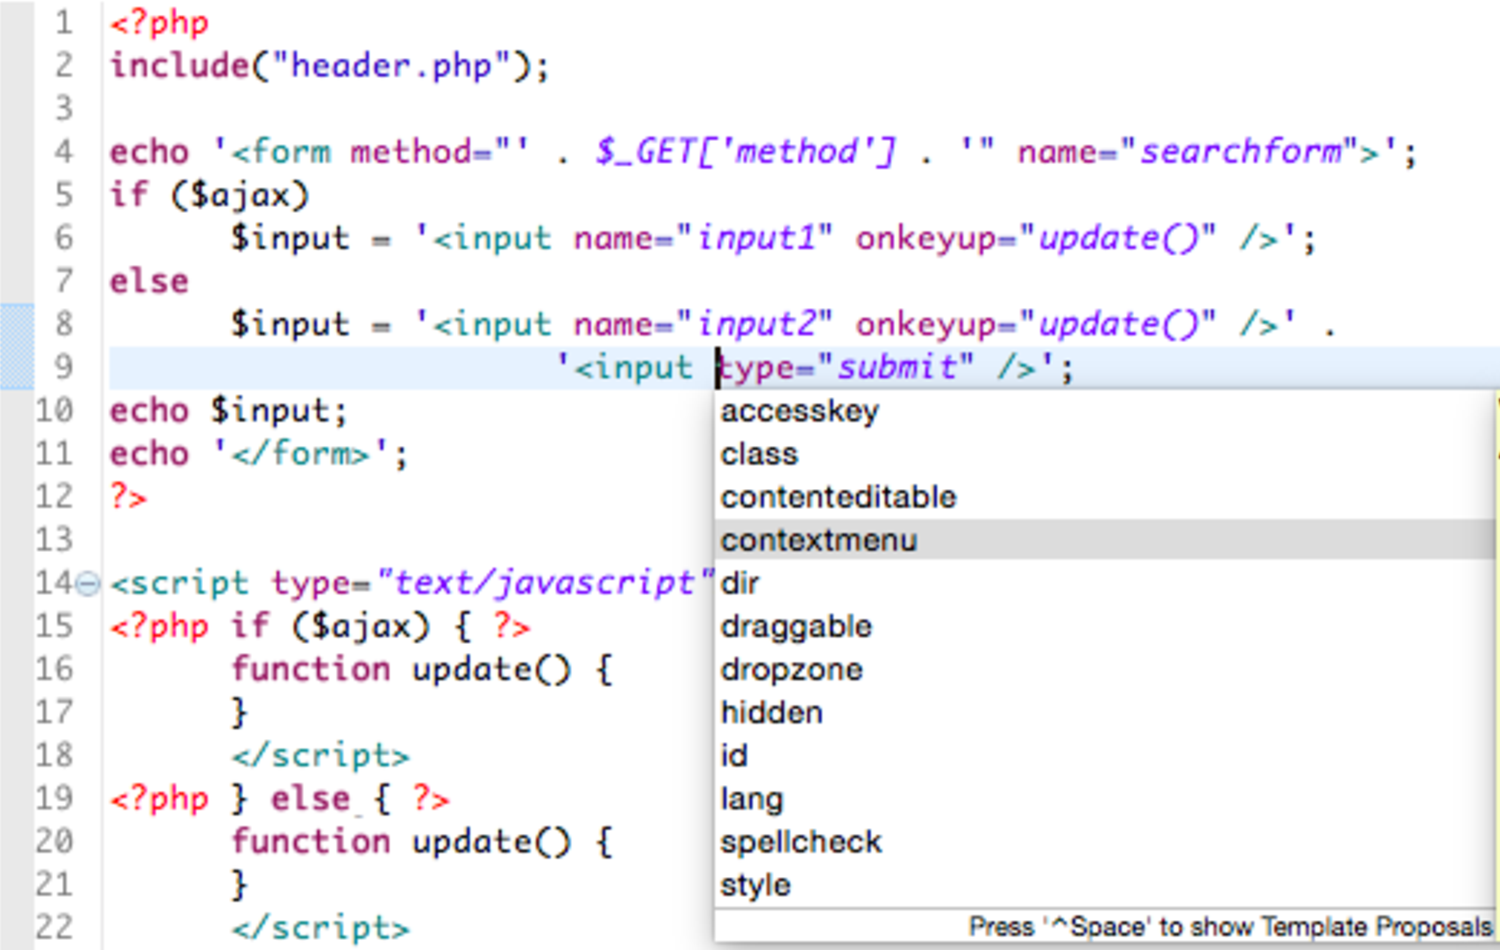
\includegraphics[width=.9\textwidth]{pics/Varis.pdf}
\caption{Пример функциональности Varis: автодополнение и подсветка синтаксиса во встроенном HTML в среде разработки Eclipse}
\label{fig:method} 
\end{center}
\end{figure}


{\footnotesize
  \centering
  
  \begin{longtable}{| r | p{2cm} | p{3cm} | p{2.5cm} | p{7.5cm} |}
  
  \hline                               
  \hline
  \textnumero & Шаг & Вопрос & Необходимые ресурсы & Что должен содержать ответ \\
  \hline 
  \multirow{2}{*}1 
  &
  \multirow{2}{*}{\begin{minipage}{2cm}Анализ целей и задач\end{minipage}}
  &
  Что нужно сделать
  & 
  Задачи
  &
  Список задач, при решении которых необходимо обрабатывать строковые выражения.
  \\  
  & 
  &
  Зачем
  &
  Цели
  &
  Планируется ли модификация и сопровождение
  \\
  \hline
  \multicolumn{5}{|p{17cm}|}{\centering Дальнейшие шаги выполняются, если список задач, требующих обработку строковых выражений не пуст.}\\
  \hline
  \multirow{2}{*}2 
  &
  \multirow{2}{*}{\begin{minipage}{2cm}Первичный анализ системы.\end{minipage}}
  &
  Сколько в системе строковых выражений, требующих обработки.
  & 
  Исходный код системы.
  &
  Количество точек интереса. 
  \\  
  & 
  &
  На сколько сложные строковые выражения используются.
  &
  Исходный код системы.
  &
  Количество операторов для каждой точки интереса, участвующих в формировании соответствующего запроса.
  \\
  \hline
 
  \multirow{3}{*}3 
  &
  \multirow{3}{*}{\begin{minipage}{2cm}Доступ к исходной сиситеме в реальных условиях.\end{minipage}}
  &
  Важность наличия доступа.
  &
  Список задач, требующих обработки строковых выражений. Наличие динамики.
  &
  Есть ли задачи, решение которых упрощается при наличии доступа к работающей системе. Можно ли их решать при его отсутствии.
  \\  
  & 
  &
  Что доступно на чтение.
  &
  Заказчик.
  &
  Какие данные и в каком объёме можно получать от работающей системы.
  \\
  & 
  &
  Какие изменения возможно вносить в работающую систему.
  &
  Заказчик.
  &
  Какого рода изменения и в какие модули можно вносить.
  \\
  \hline
 
  \multirow{3}{*}4 
  &
  \multirow{3}{*}{\begin{minipage}{2cm}Роль строковых выражений в обрабатываемой системе.\end{minipage}}
  &
  А надо ли
  & 
  Список задач
  &
  Есть ли задачи, отражаюиеся на рантайме
  \\  
  & 
  &
  для чего используется
  &
  Код, документация, заказчик
  &
  Для каждой точки выполнения количество операторов, участвующих в формировании соответствующего запроса.
  \\
  & 
  &
  На сколько активно используется.
  &
  Код, документация, заказчик
  &
  Статичесикие и динамические показатели. Сколько точек интереса, на сколько интенсивно выполняется, на сколько производительность данной компоненты критична.
  \\
  \hline
 
  \multirow{4}{*}5 
  &
  \multirow{4}{*}{\begin{minipage}{2cm}Анализ вычислительных ресурсов\end{minipage}}
  &
  А надо ли
  & 
  Список задач
  &
  Есть ли задачи, отражаюиеся на рантайме
  \\  
  & 
  &
  На сколько критичен дфк
  &
  роль дфк
  &
  Для каждой точки выполнения количество операторов, участвующих в формировании соответствующего запроса.
  \\
  & 
  &
  Как можем оценить
  &
  доступ к системе
  &
  Для каждой точки выполнения количество операторов, участвующих в формировании соответствующего запроса.
  \\
  & 
  &
  Есть ли запас
  &
  Заказчик
  &
  Для каждой точки выполнения количество операторов, участвующих в формировании соответствующего запроса.
  \\
  \hline
 
  \multirow{3}{*}6 
  &
  \multirow{3}{*}{\begin{minipage}{2cm}Особенности\end{minipage}}
  &
  Зачем
  & 
  список задач
  &
  Надо знать, на какие особенности обращать внимание.
  \\  
  & 
  &
  Существуют ли впринципе
  &
  Список задач, знания языков
  &
  Список особенностей
  \\
  & 
  &
  Есть ли в системе
  &
  код
  &
  Список особенностей
  \\
  \hline
 
  \multirow{6}{*}7 
  &
  \multirow{6}{*}{\begin{minipage}{2cm}Выбор подхода.\end{minipage}}
  &
  Сопровождение результатов
  & 
  цели
  &
  Есть ли задачи, отражаюиеся на рантайме
  \\  
  & 
  &
  Доступ к системе
  &
  доступ к системе
  &
  Для каждой точки выполнения количество операторов, участвующих в формировании соответствующего запроса.
  \\
  & 
  &
  Доступность ресурсов
  &
  анализ ресурсов
  &
  Для каждой точки выполнения количество операторов, участвующих в формировании соответствующего запроса.
  \\
  & 
  &
  Точность
  &
  Задачи
  &
  Для каждой точки выполнения количество операторов, участвующих в формировании соответствующего запроса.
  \\
  & 
  &
  Особености
  &
  Особенности
  &
  Есть ли особенности, влияющие на выбор подхода.
  \\
  & 
  &
  Задачи
  &
  Срисок задач
  &
  Для каждой точки выполнения количество операторов, участвующих в формировании соответствующего запроса.
  \\
  \hline
 
  \multirow{4}{*}8 
  &
  \multirow{4}{*}{\begin{minipage}{2cm}Составление рекомендаций по выбору инструмента.\end{minipage}}
  &
  Требуется ли внутреннее представление
  & 
  Задачи
  &
  Есть ли задачи, отражаюиеся на рантайме
  \\  
  & 
  &
  Сложные случаи
  &
  Особенности
  &
  Для каждой точки выполнения количество операторов, участвующих в формировании соответствующего запроса.
  \\
  & 
  &
  Динамика, статика
  &
  подход
  &
  Для каждой точки выполнения количество операторов, участвующих в формировании соответствующего запроса.
  \\
  & 
  &
  Точность
  &
  Заказчик
  &
  Для каждой точки выполнения количество операторов, участвующих в формировании соответствующего запроса.
  \\

  
  \hline
  \hline
  \caption{Основные шаги по подготовке к реинжинирингу системы, содержащей строковые выражения, требующие обработки}\label{tbl:method}
  \end{longtable}
}


\begin{enumerate}
  \item \textbf{Анализ целей и задач.}
  
  Проанализировать цели и задачи. От того, какие задачи необходимо решать, напрямую зависит выбор средств и инструментов. Основные классы задач затрагивающих динамически формируемый код, которые можно выделить на данном этапе, приведены ниже.
  
  \begin{itemize}
    \item Оценка качества кода и его сложности, что часто сводится к подсчёту некоторых формальных метрик кода~\cite{SoftwareMetrics, DSQLQualityMesureBIG}. Необходимо определить, требуется ли построение структурного представления кода для вычисления требуемых метрик с необходимой точностью.
    \item Анализ надёжности системы, поиск различного рода уязвимостей и ошибок. Требуется изучение типов ошибок, которые предполагается обнаруживать: обнаружене некоторых типов ошибок требуют построения структурного представления кода (семантические ошибки), в то время, как для других это не требуется (лексические, синтаксические ошибки).
    \item Извлечение или восстановлении утраченных знаний о системе и её изучение.
    \item Трансформация исходной системы: рефакторинг, перенос на новые программно-аппаратные системы.
  \end{itemize}
  
  При этом необходимо проанализировать конечные цели реинжиниринга. Особенно важен данный шаг при необходимости решать задачи трансформации динамически формируемого кода. Например, если целью является как можно более быстрое получение работающей системы, дальнейшее развитие которой не планируется, то можно пожертвовать качеством кода результирующей системы, что может существенно упростить её обработку. Однако, если после выполнения трансформаций планируется активная разработка или поддержка полученной системы, то необходимо получить результирующий код как можно более привычный для разработчиков системы. Это упростит дальнейшую работу с ним, позволит уменьшить затраты на обучение команды, поиск новых специалистов.
  
  Например, при трансляции хранимого SQL-кода, активно использующего динамический SQL, с одного языка на другой, важно сохранить однородность. Особенно если планируется дальнейшее развитие системы. Это обусловлено тем, что различные диалекты SQL содержат большое количество особенностей и разработчики на SQL часто оказываются специалистами достаточно узкого профиля. Таким образом, наличие двух различных диалектов в место одного, может усложнить набор команды. Более того, в процессе разработки необходимость переключаться между несколькими диалектами так же может вызвать трудности.
  
  Таким образом, необходимо ответить на следующий вопрос: планируется ли активное изменение системы после её реинжиниринга, если он включает трансформации.
  
  \item \textbf{Первичный анализ проекта.} На данном этапе необходимо проанализировать исходный код системы и выяснить характеристики встроенного текстового кода. Для этого, как правило, можно использовать стандартные средства анализа программного кода. Однако, скорее всего они будут требовать модификации, по этому необходимо иметь доступ к исходному коду. Необходимо оценить следующие характеристики.
  \begin{itemize}
    \item Клоичество точек выполнения встроенного кода. Как правило, за выполнение выражений на встроенном языке отвечают характерные языковые конструкции, например \verb|EXECUTE|\footnote{Конструкция язука T-SQL, позволяющая выполнить динамически формируемый запрос. Документация: \url{https://msdn.microsoft.com/en-us/library/ms188332.aspx}. Посешён 29.07.2015.} в языке T-SQL. следовательно, необходимо оценить количество таких конструкций. Для грубой оценки можно использовать простой текстовый поиск (если такой поиск говорит о полном отсутствии конструкций, то дальнейший анализ можно не проводить). Для более точной оценки необходимо использовать структурное представление кода, чтобы, например, не учитывать код, находящийся в комментариях. Получить структурное представление и доступ к нему можно с помощью библиотек синтаксического анализа соответствующего языка.
    
    \item Сложность формирования строковых выражений. Прежде всего необходимо определить наличие динамически формируемого кода и оценить сложность его формирования, так как в случае использования только константных строковых литералов не потребуется специальных инструментов для анализа встроенного кода.
    
    Для данной оценки можно использовать протягивания констант. Его необходимо модифицировать таким образом, чтобы он отдельно обрабатывал выражения, отвечающие за формирование кода, и собирал о них следующую информацию о процессе формирования кода как для каждой точки выполнения, так и для всей системы вцелом.
    \begin{itemize}
      \item Количество конкатенаций.
      \item Количество операторов ветвления: \verb|if-then-else|, \verb|switсh-case| и т.д.
      \item Количество строковых функций: \verb|replace|, \verb|substring| и т.д.
      \item Количество циклов, как ``явных'' (\verb|while|, \verb|for|), так и организованных с помощью рекурсии.
      \item Количество переменных, значение для которых нельзя полностью вычислить статически (например, они получают значение из пользовательского входа).
      \item Факт формирования кода в телах более чем одного метода/процедуры. Необходимость межпроцедурного анализа.
    \end{itemize}
  \end{itemize}
  
  \item \textbf{Роль динамически формируемого кода в системе.} На данном шаге необходимо определить, какую роль в функционировании системы играют динамически формируемые запросы. Возможны следующие существенно различные ситуации.
  \begin{itemize}
    \item Использование динамически формируемого кода является один из основных элементов дизайна системы. Данная ситуация, как правило, выделяется большим количеством точек исполнения и наличием сложно формируемого кода. Важно определить, каие именно компонениты системы построены таким образом, так как использование встроенных языков может быть весьма неоднородным. Средние значения по всей системе могут быть не велики, при этом ряд ключевых компонент построены с активным использованием динамически формируемого кода, а в остальных он отсутствует. При этом может оказаться, что ключевые компоненты являются ещё и самыми критическими по производительности учестками системы.
    
    \item Динамически формируемый код используется как вспомогательное средство. Чаще всего явным признаком такой ситуации является его малое количество или полное отсутствие. Однако, это не всегда так. Возможна ситуация, когда динамически формируемых код достаточно активно используется для реализации служебной и вспомогательной функциональности. Тот факт, что данная функциональность не является основной для системы, может позволить обращать меньше внимания, например, на производительность результатов трансформации соответствующего кода.
  \end{itemize}
  
  \item \textbf{Возможности доступа к исходной системе в реальных условиях.} Возможность изучения системы в реальных условиях может дать большое количество полезной информации, которую трудно или дажен невозможно получить другими способами, так как даже тесты часто не воспроизводят реальное функционирование системы. Однако он часто оказывается невозможным или крайне затруднённым, что вызывается, с одной стороны вопросами безопасности, с другой стороны надёжностью, так как гарантировать, что внесённые изменения не отразатся на работоспособности системы часто затруднительно.  
  \begin{itemize}
    \item Есть ли доступ к системе, работающей в реальных условиях? Чтение определённых журнальных файлов, перехват сообщений на каком-либо уровне, доступ к реальной базе данных.
    \item Возможен ли запуск модифицированной системы в реальных условиях? Если мы можем запустить модифицированную систему, то важно убедиться, что будет возможность получить обратно собранную информацию.
    \item Модификации какого рода разрешены? Что можно собирать, а что нельзя.
  \end{itemize}
  
  \item \textbf{Анализ требований к производительности и потреблению ресурсов.} Необходимо определить, можем ли мы позволить себе дополнительные накладные расходы. Ответ на данный вопрос особенно важен при выборе между статическим и динамическим подходом к трансляции динамически формируемого кода. Выполнение динамически формируемых SQL-запросов само по себе требует дополнительных ресурсов. Если на предыдущих шагах было выяснено, что динамически формируемый код активно используется в критическом по произволительности месте, а вычислительные ресурсы ограничены, то применение динамичекого подхода, требующего дополнительных вычислений во время выполнения, может существенно ухудшить быстродействие системы.
  
  \item \textbf{Анализ особенностей конкретного вншнего и встроенного языков.} Многие задачи требуют комплексной обработки внешнего и встроенного кода. Например, при статическом поиске ошибок, включающем ошибки использования типов переменных, необходимо проводить анализ, проверяющий, что тип переменной во внешнем коде соответствует типу, возвращаемому запросом. Пример несовпадения типов приведён в листинге~\ref{lst:typeChecking}: : переменная \texttt{result} имеет тип \texttt{List<string>}, однако запрос возвращает коллекцию двухэлементных кортежей.
  
\fvset{frame=lines,framesep=5pt}
\begin{listing}
    \begin{pyglist}[language=csharp,numbers=left,numbersep=5pt]

public List<string> NewReport
  (int prodId = 0, int status = 0, int nType = 0)
{
    int nProdIdL = prodId;

    string sMagicKey = "[" + prodId.ToString() + "]";

    string tbl = status == 0 ? "InOrders " : "OutOrders ";

    while (nProdIdL > 0)
    {
        sMagicKey = "[" + sMagicKey + "]";
        nProdIdL = nProdIdL - 1;
    }

    string sExec =
        "SELECT sOrderDescription, " + sMagicKey
        + " FROM ts." + tbl;

    List<string> result = db.Execute(sExec);
    return result;
}
\end{pyglist}
\caption{Пример кода метода на языке программирования C\#, в котором ожидаемый и реальный тип результата запроса не совпадают: переменная \texttt{result} имеет тип \texttt{List<string>}, однако запрос возвращает коллекцию двухэлементных кортежей}
\label{lst:typeChecking}
\end{listing}

  Наличие некоторых связей внешнего и встроенного кода делает невозможным полностью динамический подход, так как без статического анализа не будет получена информация, необходимая для корректного преобразования внешнего кода. Примером такой ситуации может служить трансформация кода хранимой процедуры с динамическими запросами, формирующими запрос \verb|SELECT| из T-SQL в PL-SQL. При этом результат данного запроса должен быть результатом процедуры. В T-SQL вне зависимости от типа сформированного запроса его выполнение производится с помощью команды \verb|EXECUTE| и результат выполнения автоматически возвращается в качестве результата процедуры, а в PL-SQL для того, чтобы получить результат выполнения запроса и вернуть его наружу из процедуры необходимо использовать конструкцию \verb|EXECUTE IMMEDIATE ... INTO out_var|~\footnote{Языковая конструкция, которая позволяетвыполнить запрос и сохранить результат его выполнения в переменной. Описание в документации по языку PL-SQL: \url{http://docs.oracle.com/cd/B12037_01/appdev.101/b10807/13_elems017.htm}. Посешён 29.07.2015.}, при этом \verb|out_var| должна быть объявлена аргументом процедуры с модификатором \verb|OUT|~\footnote{Модификатор \texttt{OUT} для аргумента подпрограммы означает его передачу по ссылке, что позволяет возвращать его значение в вызывающую подпрограмму. Описание в документация по языку PL-SQL: \url{http://docs.oracle.com/cd/A97630_01/appdev.920/a96624/08_subs.htm\#752}. Посешён 29.07.2015.}. То есть в данном случае без статического анализа динамически формируемого кода невозможно корректно преобразовать внешний код.

  Отдельно нужно проверить наличие конструкций, которые заведомо усложняют автоматическую обработку системы. Примером такой конструкции может служить \verb|MERGE|\footnote{Операция позволяющая обновременно добовлять новые записи и обновлять существующие. Описание в документации по языку PL-SQL: \url{http://docs.oracle.com/cd/B10500_01/appdev.920/a96624/13_elems30.htm}. Посешён 29.07.2015.} в PL-SQL, проекция которого в другие языки может потребовать существенных усилий.
  
  \item \textbf{Выбор подхода.} Основной вопрос, который необходимо решить на данном шаге --- это граница статического и динамического подхода. На предыдущих шагах могли быть выявлены особенности, накладывающие ограничения на выбор. Может оказаться, что необходим не чистый статический~\cite{Syrcose} или динамический~\cite{DynamicDSQLTranslation} подходы, а их смесь. Такая ситуация возникает когда решение задачи статически крайне затруднено или невозможно, но динамический подход требует неприемлимых накладных расходов. Может быть и смешанный подход. Примером может послужить обработка конструкции \verb|MERGE|, статическая прокекция которой сложна, в случае активного использования соответствующего кода. В данном случае на этапе статического анализа вычисляется вся информация, необходимая для трансформаций во время выполнения, которая может быть вычислена, и сохраняется, например, в специальных переменных. Далее, во время выполнения происходит окончательная трансформация кода в нужный вид и наличие заранее вычисленной информации сокращает накладные расходы.
  
  \item \textbf{Принятие решения.} Результатом проделаного анализа должно стать решение о том, какими именно средствами проводить анализ встроенного кода. С одной стороны, необходимо выбрать инструмен. Обзор некоторых из них приведён в разделе~\ref{SELToolsDescr} данной работы. Приведём примеры ситуаций, в которых можно использовать некоторые из них.
  \begin{itemize}
    \item Статический поиск синтаксических ошибок может быть автоматически проведён с помощью таких инструментов как JSA~\cite{JSAUrl} или PHPSA~\cite{PHPSAUrl} для сложно формируемых выражений. Для детальной диагностики может потребоваться применение инструментов типа Alvor~\cite{AlvorUrl}.
    \item Статическая трансформация встроенного кода, каждое выражение которого полностью содержится в константном литерале, может быть автоматически осуществлена SQL Ways~\cite{SQLWays}.
    \item Статическая трансформация встроенного кода со сложной логикой формирования может быть автоматизирована с помощью инструментов, разработанных на основе платформы, аналогичной представленной в данной работе.
  \end{itemize}
  
  С другой стороны необходимо провести границы автоматизации прооцесса. Провести чёткое разделение крайне сложно, так как возможны различные ситуации в диопазоне от наличия готового инструмента, решающего необходимые задачи и специалистов, умеющих с ним работать, до отсутствия инструмента и специалистов, способных его создать. В такой ситуации характеристики системы, оцененные на предыдущих шагах, не являются решающим фактором в принятии решения о ручной обработке или автомитизации и её границах, однако являются необходимым условием для принятия правильного решения. 
  
\end{enumerate}

Изложенный метод позволяет что-то там сделать и может быть адаптирован как к системам, использующим к другие встроенные языки, так и к системам с несколькими встроенными языками, так как их обработка может проводиться независимо. 



\clearpage
